\documentclass[aspectratio=169,10pt]{beamer}

\usetheme{Madrid}
\usecolortheme{default}
\usefonttheme{professionalfonts}

\usepackage{fontspec}
\setmainfont{Segoe UI}
\setsansfont{Segoe UI}
\usepackage{booktabs}
\usepackage{graphicx}
\usepackage{amsmath}
\usepackage{xcolor}
\usepackage{array}

% Custom clean academic palette
\definecolor{NavyPrimary}{RGB}{20, 48, 92}
\definecolor{TealAccent}{RGB}{13, 128, 128}
\definecolor{SoftBg}{RGB}{244, 247, 252}
\definecolor{WarmOrange}{RGB}{196, 88, 22}

\setbeamercolor{palette primary}{bg=NavyPrimary,fg=white}
\setbeamercolor{palette secondary}{bg=TealAccent,fg=white}
\setbeamercolor{palette tertiary}{bg=NavyPrimary,fg=white}
\setbeamercolor{structure}{fg=NavyPrimary}
\setbeamercolor{frametitle}{bg=NavyPrimary,fg=white}
\setbeamercolor{block title}{bg=NavyPrimary,fg=white}
\setbeamercolor{block body}{bg=SoftBg,fg=black}
\setbeamercolor{block title example}{bg=TealAccent,fg=white}
\setbeamercolor{block body example}{bg=SoftBg,fg=black}
\setbeamercolor{block title alerted}{bg=WarmOrange,fg=white}
\setbeamercolor{block body alerted}{bg=SoftBg,fg=black}

\setbeamertemplate{navigation symbols}{}
\setbeamertemplate{footline}[frame number]

\title[Hybrid-v3: Codec-Bypass Audio Restoration]{\textbf{Hybrid-v3: Kết Hợp Bộ Lọc Tuyến Tính \& Mô Hình Sinh}\\ \large Cải Thiện Chất Lượng Phục Hồi Âm Nhạc Trên Nền SonicMaster}
\author{Nhóm Tái Lập \& Mở Rộng SonicMaster}
\date{Ngày 23 tháng 11 năm 2026}

\begin{document}

%---------------------------------------------------------
\begin{frame}
  \titlepage
\end{frame}

%---------------------------------------------------------
\begin{frame}{1. Bối Cảnh: Vì Sao SonicMaster Bị Mờ Chi Tiết \& Giọng ``Kim Loại''?}
  \begin{columns}[T]
    \begin{column}{0.54\textwidth}
      \footnotesize
      \begin{block}{Cơ chế của mô hình sinh SonicMaster ($A_0$)}
        \begin{itemize}
          \item \textbf{Đầu vào ($x$):} Bản nhạc lỗi + câu lệnh mô tả lỗi cần sửa.
          \item \textbf{Quy trình 3 bước:} Sóng âm $x$ $\rightarrow$ \textbf{Bộ nén (VAE Encoder)} $\rightarrow$ Mô hình khuếch tán sửa lỗi $\rightarrow$ \textbf{Bộ giải nén (VAE Decoder)} $\rightarrow$ Đầu ra $s$.
        \end{itemize}
      \end{block}
      \begin{alertblock}{Điểm nghẽn ở bước nén / giải nén VAE}
        \begin{itemize}
          \item Bộ nén VAE thu gọn âm thanh xuống tốc độ khung rất thấp ($21{,}53\text{ Hz}$, giảm mẫu $2048\times$).
          \item Quá trình nén--giải nén làm \textbf{mất độ sắc nét của pha và họa âm mịn}: ngay cả khi cho nhạc sạch đi qua VAE, \textbf{Mel-SSIM tụt còn $0{,}546$} và giọng hát xuất hiện cảm giác \textbf{``kim loại'' / robot}.
        \end{itemize}
      \end{alertblock}
    \end{column}
    \begin{column}{0.43\textwidth}
      \footnotesize
      \begin{exampleblock}{Ý tưởng cốt lõi của Hybrid-v3}
        \textbf{Không lấy thẳng sóng âm của $s$ khi không cần thiết.}
        \begin{enumerate}
          \item Coi $s$ ($A_0$) là \textbf{``bản mẫu mục tiêu''} (biết AI muốn cân bằng tần số, âm lượng, độ động ra sao).
          \item Dùng \textbf{bộ lọc DSP truyền thống} chỉnh trực tiếp lên \textbf{sóng gốc $x$} để tránh đi qua VAE.
        \end{enumerate}
      \end{exampleblock}
      \vspace{0.4em}
      \centering
      \begin{tabular}{lc}
        \toprule
        \textbf{Nhánh (Test 7.000 mẫu)} & \textbf{Mel-SSIM} $\uparrow$ \\
        \midrule
        Input ($x$) & 0.777 \\
        VAE Roundtrip & 0.546 \\
        SonicMaster ($A_0$) & 0.609 \\
        \bottomrule
      \end{tabular}
    \end{column}
  \end{columns}
\end{frame}

%---------------------------------------------------------
\begin{frame}{2. Suy Hao Tuyến Tính Là Gì \& Vì Sao DSP Chỉnh Lại Được?}
  \footnotesize
  \begin{block}{Định nghĩa trực quan: Suy hao tuyến tính (Linear Degradations)}
    Là những lỗi \textbf{chỉ làm thay đổi tỷ lệ năng lượng hoặc độ lớn} giữa các vùng tần số, giữa hai kênh trái/phải, hoặc theo thời gian — \textbf{không phá hủy hay xóa mất thông tin gốc của sóng âm $x$}:
    \begin{itemize}
      \item \textbf{Sai màu âm (EQ):} Quá tối (\texttt{dark}), chói (\texttt{bright}), đục (\texttt{mud}), ù trầm (\texttt{boom}), thiếu ấm (\texttt{warm}), mờ (\texttt{clarity}), thiếu thoáng (\texttt{airy}), màu micro (\texttt{mic}).
      \item \textbf{Sai âm lượng, độ động \& không gian:} To/nhỏ (\texttt{volume}), bị nén phẳng (\texttt{comp}), mất lực nảy (\texttt{punch}), hẹp 2 kênh (\texttt{stereo}).
    \end{itemize}
  \end{block}
  \begin{columns}[T]
    \begin{column}{0.48\textwidth}
      \begin{exampleblock}{Vì sao điều chỉnh lại được trên sóng gốc $x$?}
        \begin{itemize}
          \item Các lỗi này có tính \textbf{khả nghịch}: chỉ cần biết mức lệch giữa $x$ và bản mẫu $s$, bộ lọc DSP tính ngược lại được đường cong bù trừ.
          \item Xử lý trực tiếp trên $x$ $\Rightarrow$ \textbf{bảo toàn 100\% pha và họa âm gốc}, triệt tiêu hoàn toàn tiếng kim loại của VAE.
        \end{itemize}
      \end{exampleblock}
    \end{column}
    \begin{column}{0.48\textwidth}
      \begin{block}{Chuỗi 4 bước chỉnh DSP (\texttt{peq\_P})}
        \begin{enumerate}
          \item \textbf{EQ 8 băng tần:} Cân bằng lại dải trầm--trung--cao.
          \item \textbf{Dynamics:} Khớp độ nén / độ nảy theo $s$.
          \item \textbf{Stereo (M/S):} Cân lại độ rộng hai loa trái/phải.
          \item \textbf{Loudness (LUFS):} Chuẩn hóa độ to tổng thể.
        \end{enumerate}
      \end{block}
    \end{column}
  \end{columns}
\end{frame}

%---------------------------------------------------------
\begin{frame}{3. Suy Hao Phi Tuyến Là Gì \& Vì Sao Phải Dựa Vào Mô Hình Sinh?}
  \footnotesize
  \begin{alertblock}{Định nghĩa trực quan: Suy hao phi tuyến / Mất thông tin}
    Là những lỗi mà \textbf{tín hiệu gốc đã bị trộn lẫn phức tạp hoặc bị cắt mất dữ liệu}, nên các bộ lọc tuyến tính đơn giản (tăng/giảm tần số) \textbf{không thể đảo ngược}:
    \begin{itemize}
      \item \textbf{Vang phòng (\texttt{reverb}: \texttt{small}, \texttt{big}, \texttt{mix}, \texttt{real}):} Âm thanh bị dội lặp lại hàng nghìn lần và làm xáo trộn pha ($\text{phase\_corr}$ tụt xuống $\approx 0{,}23$).
      \item \textbf{Méo cắt đỉnh (\texttt{clip}):} Đỉnh sóng bị xén phẳng lì $\rightarrow$ phát sinh tần số hài giả (rè/vỡ) không có trong bản gốc.
      \item \textbf{Mất hẳn dải tần (\texttt{xband}):} Một vùng tần số bị cắt về $0$ (nhân hệ số EQ lên vẫn bằng $0$).
      \item \textbf{Suy giảm quá sâu ($> 24\text{ dB}$):} Tín hiệu gốc chìm sát nền nhiễu lượng tử hóa 16-bit; kéo to lên sẽ khuếch đại tiếng xì nền.
    \end{itemize}
  \end{alertblock}
  \begin{block}{Kết luận thiết kế}
    Với nhóm lỗi phi tuyến, chỉ \textbf{mô hình sinh (SonicMaster $A_0$)} mới có khả năng suy đoán và tái tạo lại phần thông tin đã mất hoặc tách bỏ đuôi vang $\Rightarrow$ Hybrid-v3 chủ động \textbf{fallback về $s$ ($A_0$)} hoặc \textbf{chỉ lấy phần dải tần bị mất từ $s$}.
  \end{block}
\end{frame}

%---------------------------------------------------------
\begin{frame}{4. Kiến Trúc Tổng Thể \& Phân Nhánh Của Hybrid-v3 (6.720 Mẫu Confirm)}
  \begin{columns}[c]
    \begin{column}{0.55\textwidth}
      \centering
      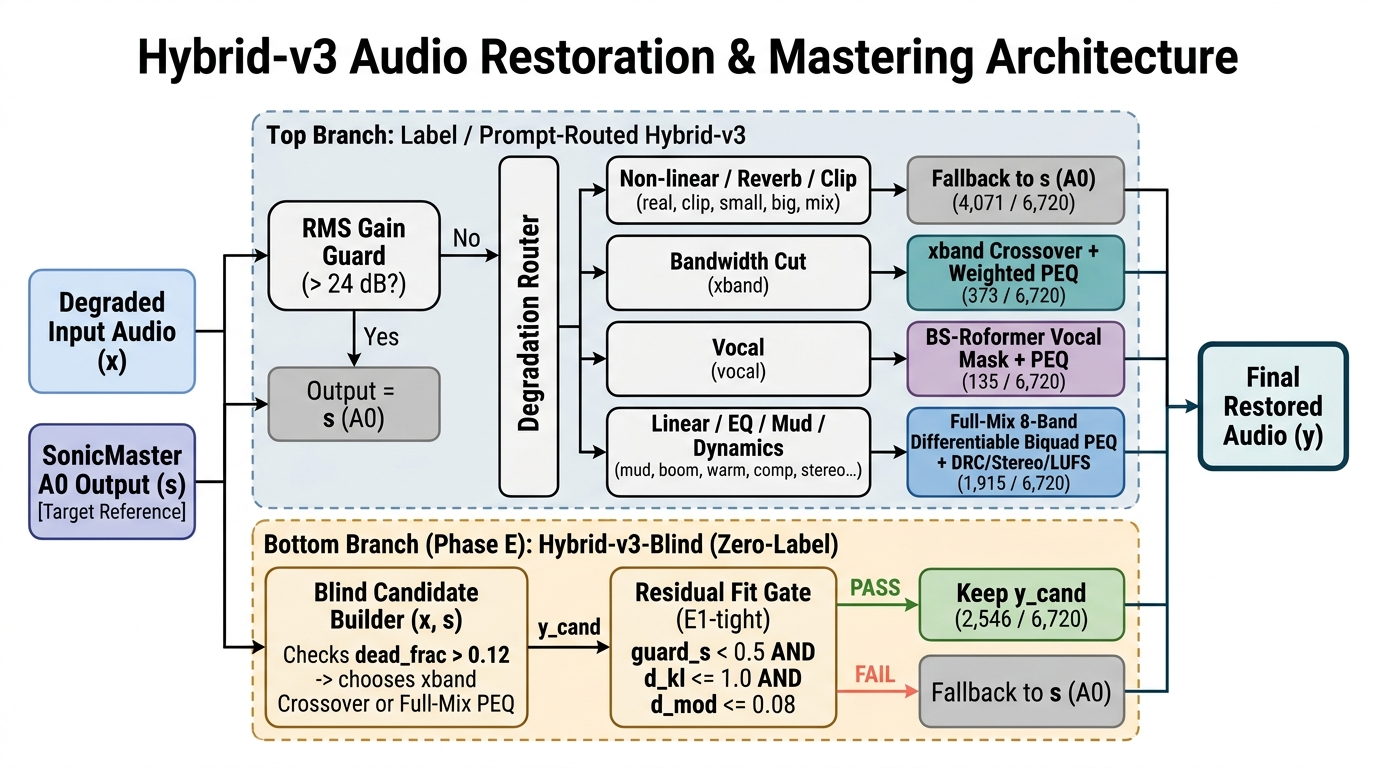
\includegraphics[width=\textwidth,height=0.68\textheight,keepaspectratio]{artifacts/10_extension/figures/hybrid_v3_architecture.jpg}
    \end{column}
    \begin{column}{0.43\textwidth}
      \footnotesize
      \begin{block}{5 nhánh xử lý trên Confirm (6.720 mẫu)}
        \begin{enumerate}
          \item \textbf{\texttt{S\_guard} (226):} Chênh RMS $> 24\text{ dB}$ $\rightarrow$ giữ $A_0$.
          \item \textbf{\texttt{S} Fallback (4.071):} Phi tuyến (\texttt{reverb}, \texttt{clip}) $\rightarrow$ giữ $A_0$.
          \item \textbf{\texttt{peq\_P} (1.915):} Tuyến tính $\rightarrow$ PEQ 8 băng + DSP trên $x$.
          \item \textbf{\texttt{xband\_crossover} (373):} Ghép vùng $x$ sống + vùng mất từ $s$.
          \item \textbf{\texttt{vocal\_mask\_P} (135):} Tách giọng BS-Roformer, trộn $[0{,}2, 0{,}8]$.
        \end{enumerate}
      \end{block}
      \textit{Tổng:} \textbf{2.423 mẫu} được DSP xử lý (không fallback $A_0$); \textbf{4.297 mẫu} giữ $A_0$.
    \end{column}
  \end{columns}
\end{frame}

%---------------------------------------------------------
\begin{frame}{5. Cơ Chế Từng Nhánh DSP Cốt Lõi \& Cách Gộp Thành Hệ Thống}
  \begin{columns}[c]
    \begin{column}{0.51\textwidth}
      \centering
      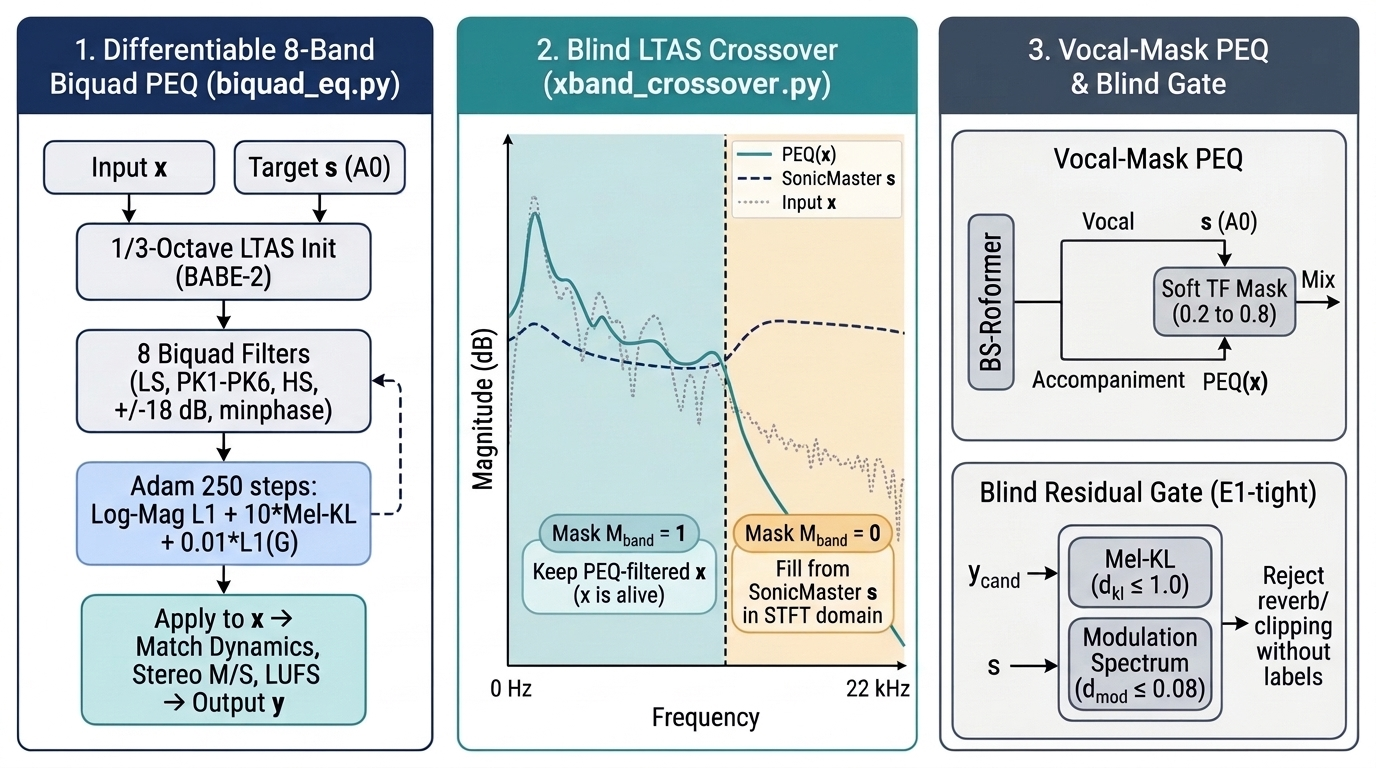
\includegraphics[width=\textwidth,height=0.68\textheight,keepaspectratio]{artifacts/10_extension/figures/hybrid_v3_dsp_details.jpg}
    \end{column}
    \begin{column}{0.47\textwidth}
      \scriptsize
      \begin{itemize}
        \item \textbf{Nhánh \texttt{peq\_P} (8-Band Differentiable Biquad PEQ):}
          Mô phỏng bàn EQ 8 nút mượt mà (\texttt{LS}, \texttt{HS}, \texttt{PK1..6}), khởi tạo theo phổ LTAS kiểu BABE-2, tối ưu 250 bước Adam hàm loss $\text{L1}_{\text{log-mag}} + 10\,\text{KL}_{\text{mel}} + 0{,}01\|G\|_1$ ($\pm 18\text{ dB}$, \texttt{minphase}) để vừa khớp $s$ vừa \textbf{chống lệch KL} (khắc phục lỗi răng cưa 128-band của v2).
        \item \textbf{Nhánh \texttt{xband\_crossover}:}
          Tính mặt nạ phổ mù $M_{\text{band}}(f)\in[0,1]$: dải nào $x$ còn sống ($M\approx 1$) thì giữ $x$ đã PEQ; dải nào $x$ bị cắt chết ($M\approx 0$) thì ghép phổ từ $s$ vào trong miền STFT.
        \item \textbf{Nhánh \texttt{vocal\_mask\_P}:}
          Dùng \texttt{BS-Roformer} tách vocal/nhạc nền trên $s$, trộn mềm $M\in[0{,}2, 0{,}8]$ để sửa cân bằng giọng mà không méo nhạc đệm.
        \item \textbf{Biến thể không cần nhãn (\texttt{Hybrid-v3-Blind}):}
          Tự chạy thử DSP tạo $y_{\text{cand}}$ rồi kiểm tra qua cổng \texttt{E1-tight} ($d_{\text{kl}}\le 1{,}0 \land d_{\text{mod}}\le 0{,}08$); nếu khớp $s$ thì giữ ($2.546$ mẫu), ngược lại trả về $s$.
      \end{itemize}
    \end{column}
  \end{columns}
\end{frame}

%---------------------------------------------------------
\begin{frame}{6. Kết Quả Metric Trên Các Mẫu KHÔNG Fallback $A_0$ ($n = 2.423$ Mẫu)}
  \begin{columns}[T]
    \begin{column}{0.48\textwidth}
      \scriptsize
      \begin{block}{Mức cải thiện trên 2.423 mẫu thực sự đổi WAV}
        Vì $4.297$ mẫu fallback có $\Delta = 0$ so với $A_0$, toàn bộ mức tăng trên tập Confirm đến từ \textbf{2.423 mẫu} (\texttt{peq\_P} + \texttt{xband} + \texttt{vocal}):
        \begin{itemize}
          \item \textbf{Mel-SSIM:} Tăng trung bình \textbf{$\mathbf{+0{,}3051}$} điểm so với $A_0$!
          \item \textbf{KL$\times$1000:} Gần như không đổi ($\Delta = +0{,}0176$).
          \item \textbf{Audiobox PQ:} Tăng nhẹ \textbf{$\Delta = +0{,}0063$} (trên $2.649$ mẫu trong \texttt{changed\_pq\_fad.npz}, $\text{PQ}_{\text{V3}} = \mathbf{7{,}7947}$).
        \end{itemize}
      \end{block}
      \begin{exampleblock}{Nhóm Single ($n=3.840$, đa số là tuyến tính)}
        \textbf{SSIM:} $0{,}6242 \rightarrow \mathbf{0{,}7804}$ ($+0{,}1562$)\\
        \textbf{KL$\times$1000:} $0{,}6923 \rightarrow \mathbf{0{,}6749}$ (tốt hơn $A_0$)\\
        \textbf{FAD-CLAP:} $0{,}0723 \rightarrow \mathbf{0{,}0267}$ (\textbf{giảm 63,1\%})\\
        \textbf{Audiobox PQ:} $7{,}7481 \rightarrow \mathbf{7{,}7670}$ ($+0{,}0189$)
      \end{exampleblock}
    \end{column}
    \begin{column}{0.49\textwidth}
      \scriptsize
      \begin{block}{Sai số từng thuộc tính tuyến tính (Confirm)}
        \centering
        \begin{tabular}{lrrrr}
          \toprule
          \textbf{Lỗi} & \textbf{n} & \textbf{Input} & \textbf{$A_0$} & \textbf{Hybrid-v3} \\
          \midrule
          \texttt{comp} & 1.143 & 0.0490 & 0.0193 & \textbf{0.0175} \\
          \texttt{punch} & 433 & 0.1428 & 0.0879 & \textbf{0.0815} \\
          \texttt{bright} & 342 & 0.0136 & 0.0061 & \textbf{0.0060} \\
          \texttt{airy} & 216 & 0.0049 & 0.0018 & \textbf{0.0018} \\
          \texttt{vocal} & 304 & 0.2567 & 0.0629 & \textbf{0.0625} \\
          \texttt{mud} & 368 & 0.4721 & 0.0473 & 0.0539 \\
          \texttt{xband} & 818 & 0.1872 & 0.0384 & 0.0421 \\
          \texttt{stereo} & 1.004 & 0.4179 & 0.1109 & 0.1151 \\
          \bottomrule
        \end{tabular}
        \vspace{0.3em}
        \\ \textit{Nhận xét:} Vượt $A_0$ ở \texttt{comp} ($-3{,}67\%$), \texttt{punch} ($-4{,}52\%$), \texttt{vocal}, \texttt{bright}, \texttt{airy}; cả \texttt{mud} ($+1{,}42\%$) và \texttt{xband} ($+2{,}02\%$) đều an toàn dưới ngưỡng $5\%$.
      \end{block}
    \end{column}
  \end{columns}
\end{frame}

%---------------------------------------------------------
\begin{frame}{7. Kết Quả Tổng Trên Toàn Bộ 6.720 Mẫu Confirm}
  \centering
  \resizebox{0.98\textwidth}{!}{%
  \begin{tabular}{lcccc}
    \toprule
    \textbf{Thước đo (Confirm)} & \textbf{$A_0$ (SonicMaster)} & \textbf{Hybrid-v2 PA1} & \textbf{Hybrid-v3} & \textbf{Hybrid-v3-Blind} \\
    \midrule
    \textbf{SSIM (All, n=6.720)} $\uparrow$ & 0.6092 & 0.6912 & \textbf{0.7192} ($+0{,}1100$) & \textbf{0.7118} ($+0{,}1026$) \\
    \quad -- Single (n=3.840) $\uparrow$ & 0.6242 & 0.7442 & \textbf{0.7804} & 0.7669 \\
    \quad -- Double+Triple (n=2.880) $\uparrow$ & 0.5891 & 0.6205 & 0.6375 & \textbf{0.6382} \\
    \midrule
    \textbf{KL$\times$1000 (All, n=6.720)} $\downarrow$ & 0.8839 & 0.9711 & \textbf{0.8902} ($1{,}007\times$) & \textbf{0.8692} ($0{,}983\times$) \\
    \quad -- Single (n=3.840) $\downarrow$ & 0.6923 & 0.7825 & \textbf{0.6749} & \textbf{0.6533} \\
    \midrule
    \textbf{FAD-CLAP (n=5.306)} $\downarrow$ & 0.0756 & 0.0466 & \textbf{0.0398} ($-47{,}4\%$) & \textbf{0.0487} ($-35{,}6\%$) \\
    \midrule
    \textbf{Audiobox PQ (n=5.306)} $\uparrow$ & 7.7103 & 7.7061 & \textbf{7.7132} ($+0{,}0029$) & 7.6093 ($-0{,}1010$) \\
    \textbf{Audiobox PQ (Full 6.720)} $\uparrow$ & 7.7075 & --- & \textbf{7.7098} ($+0{,}0023$) & 7.6275 ($-0{,}0801$) \\
    \midrule
    \textbf{Attribute Guards (19 loại)} & --- & 0 vi phạm & \textbf{0 vi phạm} & \textbf{0 vi phạm} \\
    \bottomrule
  \end{tabular}}
  \vspace{0.4em}
  \footnotesize
  \begin{exampleblock}{Tổng kết}
    \textbf{Hybrid-v3} đạt toàn bộ \textbf{5/5 tiêu chuẩn} trên cả 6.720 mẫu (vượt cả $A_0$ lẫn $PA1$ ở SSIM, FAD-CLAP, PQ và giữ KL tương đương $A_0$). \textbf{Hybrid-v3-Blind} đạt 4/5 tiêu chuẩn hoàn toàn không cần nhãn lỗi, chỉ đánh đổi nhẹ ở PQ.
  \end{exampleblock}
\end{frame}

%---------------------------------------------------------
\begin{frame}{8. Kết Luận \& Hướng Tiếp Theo}
  \footnotesize
  \begin{block}{Đóng góp chính}
    \begin{enumerate}
      \item \textbf{Phân tách rõ tuyến tính vs phi tuyến:} Suy hao tuyến tính giữ được thông tin gốc nên xử lý trực tiếp bằng DSP có tham số tối ưu từ $s$, giúp tránh hoàn toàn nút thắt VAE; suy hao phi tuyến dựa vào mô hình sinh $A_0$.
      \item \textbf{Nâng cấp từ Hybrid-v2 lên Hybrid-v3:} Thay đường cong 128-band bằng Biquad PEQ 8 băng tần có $\text{KL}_{\text{mel}}$ loss và thêm nhánh \texttt{xband\_crossover}, mở rộng phạm vi xử lý sang \texttt{mud} và \texttt{xband} (2.423 mẫu không fallback).
      \item \textbf{Hiệu quả định lượng rõ rệt:} Trên 6.720 mẫu Confirm, SSIM đạt \textbf{0.7192} ($+0{,}1100$), FAD-CLAP giảm gần một nửa (\textbf{0.0398}), Audiobox PQ \textbf{7.7132} (cao hơn $A_0$), và \textbf{0/19} vi phạm thuộc tính.
    \end{enumerate}
  \end{block}
  \begin{alertblock}{Lưu ý \& Bước tiếp theo}
    \begin{itemize}
      \item Toàn bộ số liệu trên là thước đo tự động (objective metrics + model-based PQ).
      \item Nhóm đang tiến hành \textbf{kiểm chứng nghe trực tiếp} trên các đoạn giọng hát từng ghi nhận lỗi robot/autotune để xác nhận mức độ cải thiện cảm nhận thực tế.
    \end{itemize}
  \end{alertblock}
\end{frame}

\end{document}
